\documentclass{article}
\usepackage{iclr2027_conference,times}
\usepackage[T1]{fontenc}
\usepackage[utf8]{inputenc}
\usepackage{amsmath,amssymb,amsthm,booktabs,multirow,graphicx,microtype,float,algorithm,algpseudocode,xspace}
\usepackage{hyperref}
\usepackage{svg}
\usepackage{url}
\usepackage{aliascnt}
\usepackage[nameinlink,noabbrev]{cleveref}
\hypersetup{hidelinks}

% The document is self-contained except for the bibliography, figure, and
% the two conference-style files. All tables and proofs are in this file.
\newtheorem{theorem}{Theorem}
\newaliascnt{proposition}{theorem}
\newtheorem{proposition}[proposition]{Proposition}
\aliascntresetthe{proposition}
\newaliascnt{corollary}{theorem}
\newtheorem{corollary}[corollary]{Corollary}
\aliascntresetthe{corollary}
\newcommand{\method}{\textsc{SpecGrove}\xspace}
\newcommand{\sgHigh}[1]{\textbf{#1}}
\newcommand{\sgGain}[1]{\textbf{#1}}
\newcommand{\sgMuted}[1]{#1}
\crefname{equation}{equation}{equations}
\Crefname{equation}{Equation}{Equations}
\crefname{proposition}{proposition}{propositions}
\Crefname{proposition}{Proposition}{Propositions}
\crefname{corollary}{corollary}{corollaries}
\Crefname{corollary}{Corollary}{Corollaries}
\crefname{appendix}{appendix}{appendices}
\Crefname{appendix}{Appendix}{Appendices}

\title{SpecGrove: Coordinating Speculative Trees for High-Throughput Decoding}
\author{Anonymous authors}
% Leave commented for anonymous review.
% \iclrfinalcopy

\begin{document}
\makeatletter
\typeout{LAYOUT: fontsize=\f@size pt; baseline=\the\baselineskip; parskip=\the\parskip; textwidth=\the\textwidth; textheight=\the\textheight}
\makeatother
\maketitle
% Restore the template's header outside its title box for current fancyhdr.
\ificlrfinal
  \lhead{Published as a conference paper at ICLR 2027}
\else
  \lhead{Under review as a conference paper at ICLR 2027}
\fi

\begin{abstract}
Concurrent block-diffusion speculative decoding must allocate shared verification capacity across requests that benefit differently from larger candidate trees.
We introduce SpecGrove, which jointly selects tree sizes while reusing locally generated drafts.
DFlash supplies parallel draft distributions, and a single DDTree expansion per request produces nested trees at several budgets without independently rebuilding each alternative.
The draft probability mass of added prefixes estimates the benefit of expanding a tree.
A dynamic program maximizes a priority-weighted estimate of token progress per measured verification cost for a \emph{fixed admitted request set and fixed eligible tier set}; the guarantee is a finite-set optimum of this surrogate, not an end-to-end throughput optimum.
Conditional bounds separate tier restriction, progress estimation, and cost estimation from the measured system objective.
Selected trees share one target-model pass, with attention and cached states isolated across requests.
A separate sampling analysis gives sufficient conditions for preserving the joint autoregressive output law and a perturbation bound when target conditionals differ; our BF16 implementation does not satisfy the exact-conditional premise in all audited traces.
Experiments on Qwen3-4B and Qwen3-8B span four reasoning and code-generation benchmarks under closed-batch concurrency, with comparisons using the same verifier, precision, and timing protocol.
SpecGrove improves end-to-end throughput, including online planning, by 13.0--32.1\% over DFlash.
Against a feasible fixed-45-node DDTree baseline, gains are 4.7--39.0\% at the evaluated high-concurrency setting.
Ablations attribute the largest consistent gain to adaptive tree sizing; equal and greedy adaptive-tier policies remain competitive with Bellman allocation.
On Qwen3-8B mixed workloads, \method exceeds matched TETRIS/ECHO-style allocation by 1.7--9.2\% across four fixed-concurrency cells.
In 256-request Poisson traces at a stable 2 requests/s, it matches their throughput while reducing p95 TTFT by 24.4--26.5\% and p95 end-to-end latency by 30.6--33.8\%; at an overloaded 4 requests/s, it improves median throughput by 1.7--2.2\%, with tail changes that vary by arrival trace.
Numerical audits and a separate quality study therefore bound the empirical claims rather than establishing implementation-level losslessness.
\end{abstract}

\section{Introduction}
\label{sec:introduction}
Speculative decoding reduces serial target-model invocations by verifying several proposed continuations in parallel~\citep{leviathan2023fast,chen2023accelerating}. Tree-based methods broaden the prefixes covered by one verification pass~\citep{miao2024specinfer,cai2024medusa,chen2024sequoia}. DFlash generates block-diffusion draft distributions in one pass, and DDTree turns these distributions into a high-mass candidate tree~\citep{chen2026dflash,ringel2026ddtree}. These components make branching proposals inexpensive, but a fixed budget per request does not decide how a concurrent batch should share verification capacity.

Expanding one tree changes both its request's coverage and the batch-wide verification cost. Uniformly large trees can inflate shared cost, while uniformly small trees discard useful coverage. Per-request progress therefore need not optimize aggregate progress per unit time.

Shared-budget speculation is already studied by batch schedulers such as TETRIS and ECHO~\citep{wu2025tetris,hu2026echo}; cross-request allocation is therefore not itself our novelty. \method targets a narrower systems question for \emph{branching block-diffusion drafts}: how to expose one DDTree construction as reusable capacity choices, value those choices, and pack heterogeneous trees without rebuilding independent candidates. It retains DDTree's request-local expansion order, exposes nested prefixes as discrete tiers, and chooses one eligible tier per admitted request. Selected trees share one target pass with request-local ancestry and KV state (\cref{fig:architecture}).

Covered prefix mass, service weights, and measured target cost define a per-wave surrogate rate. Bellman optimization yields the exact finite-set optimum of that surrogate for the \emph{already admitted requests and eligible tiers}; it does not optimize admission, queueing delay, or full end-to-end time. Our analysis makes these boundaries explicit by separating tier, prediction, and execution-cost errors from measured throughput.

At $C=8$, \method exceeds feasible fixed-45-node DDTree by 4.7--39.0\% at $R=384$ and DFlash by 13.0--16.8\% at $R=193$. On Qwen3-8B mixed requests, it also exceeds matched TETRIS/ECHO-style controls in all four tested capacity cells, reduces stable-load tail latency, and raises overloaded throughput under Poisson arrivals. Timing includes scheduling; ablations and quality audits delineate the operating boundaries.

\paragraph{Our contributions are:}
\begin{itemize}
\item \textbf{An executable tree-capacity interface.} Nested diffusion-draft tiers connect request-local prefix coverage to heterogeneous, request-isolated verification.
\item \textbf{Scoped optimization guarantees.} A finite-set optimum and residual certificate characterize the surrogate allocator conditional on admission and eligible tiers; approximation bounds and a causal sequence-law theorem state the assumptions needed to connect it to progress and sampling.
\item \textbf{Serving evidence across scheduler and arrival regimes.} Feasible DFlash and fixed-budget DDTree comparisons are complemented by matched TETRIS/ECHO-style controls and real-time Poisson arrivals; adaptive-tier ablations and quality audits identify where the gains arise and where simpler policies remain competitive.
\end{itemize}

\begin{figure}[t]
\centering
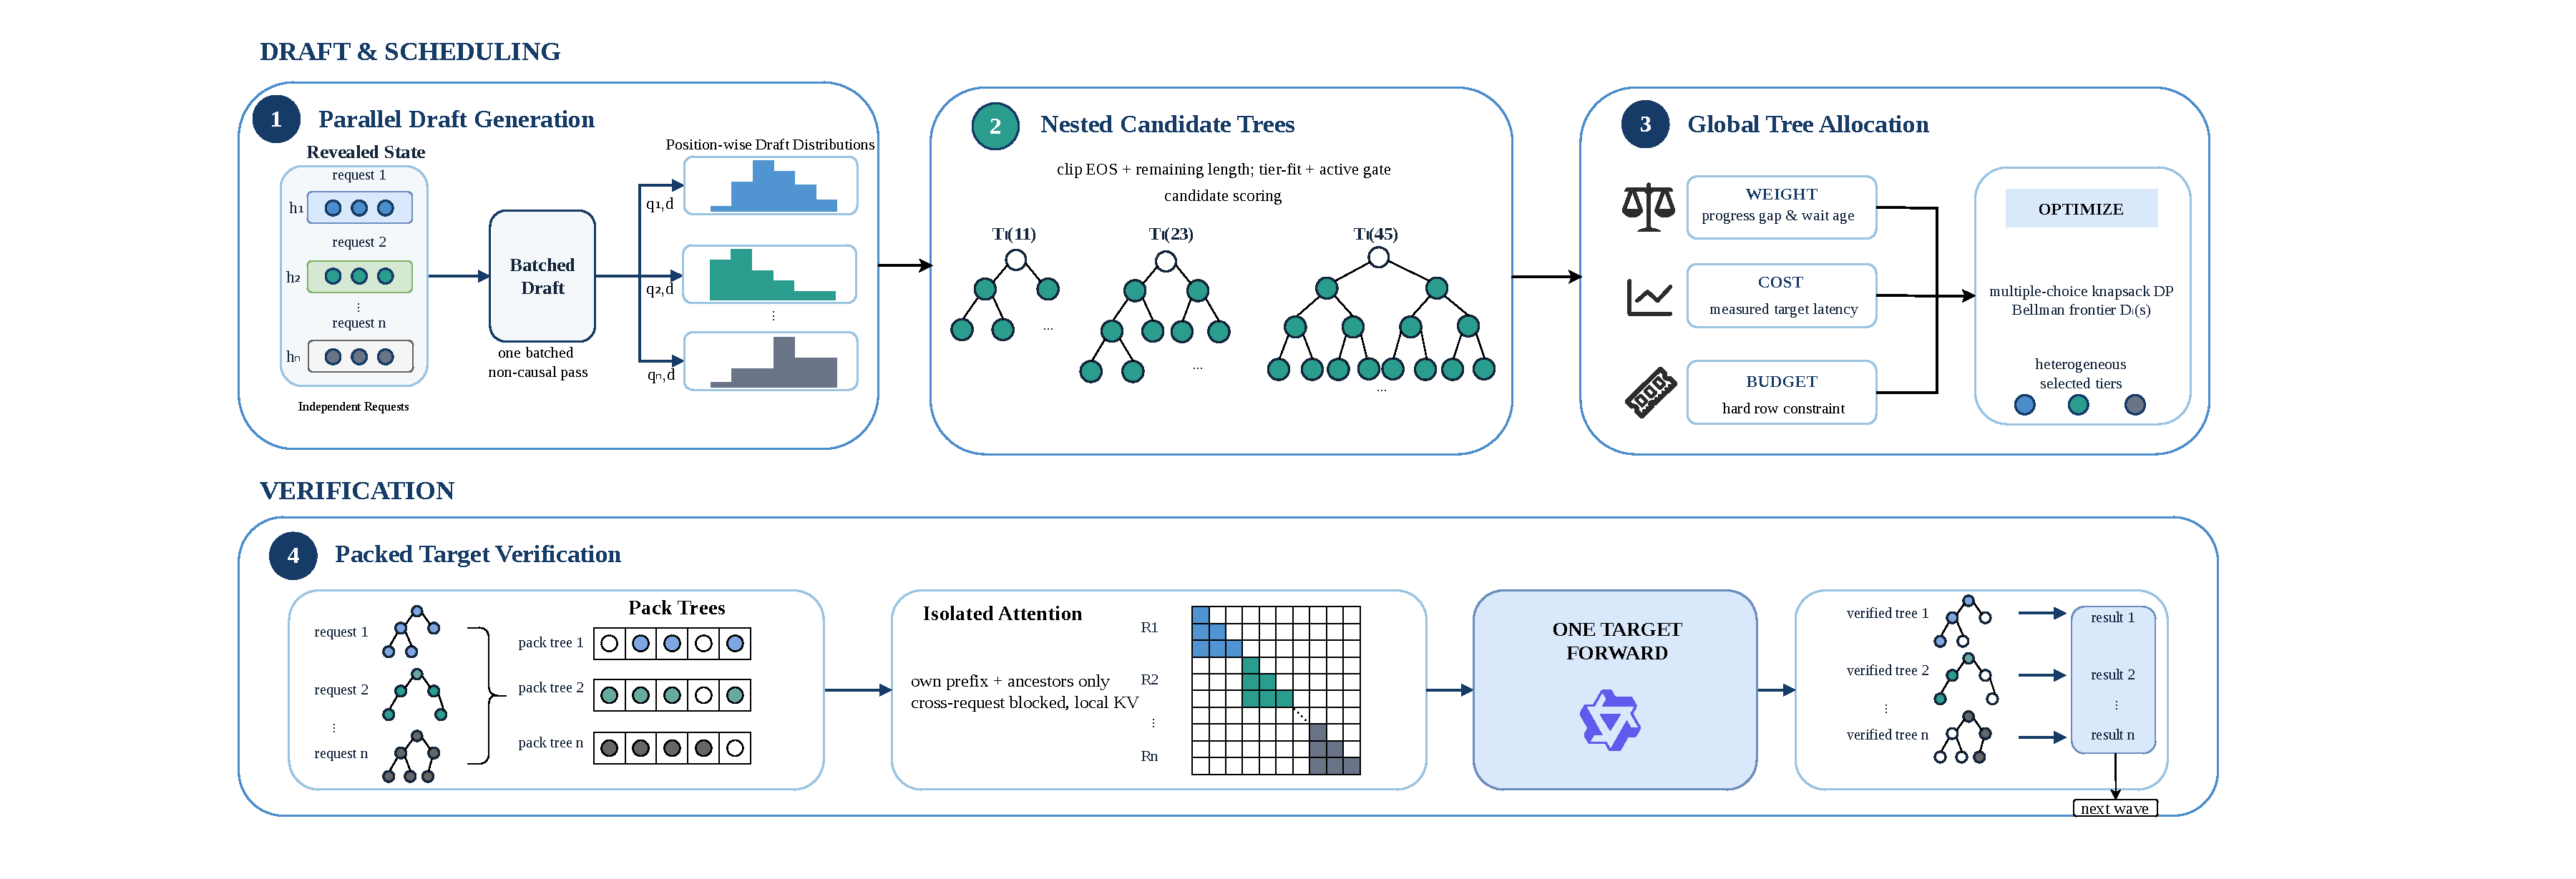
\includegraphics[width=\linewidth]{specgrove_one_scheduling_wave_editable.drawio (2).pdf}
\caption{One \method wave. Nested diffusion-draft tiers are valued by covered prefix mass and selected under a shared row budget and cost curve. Selected trees share one target pass. Each node sees its request's cached prefix, its ancestors, and itself, but no unrelated branch or request. At every visited prefix, a fresh target sample is emitted; an off-tree sample ends the wave without another draw.}
\label{fig:architecture}
\end{figure}

\section{Background and problem setting}
\label{sec:background}
\paragraph{Autoregressive and speculative generation.}
For a fixed revealed context $x$, a target model defines $p(y\mid x)=\prod_t p(y_t\mid x,y_{<t})$, with generation ending at EOS or a prescribed output cap. Conventional decoding evaluates one next-token conditional at a time. Speculative decoding uses a cheaper proposal to precompute several candidate continuations and evaluates their target conditionals together; an appropriate verification rule preserves the target law~\citep{leviathan2023fast,chen2023accelerating}. Useful progress must offset proposal and verification overhead. The tree traversal below uses fresh target sampling, rather than rejection-corrected chain sampling.

\paragraph{Block-diffusion drafts and candidate trees.}
DFlash uses target features to produce position-wise distributions $q_d$ for a future block in one draft pass~\citep{chen2026dflash}. They are not autoregressive conditionals on the tokens subsequently chosen within that block. For a continuation $v$, the product $Q(v)=\prod_{d=1}^{|v|}q_d(v_d)$ therefore defines a \emph{draft surrogate}, whereas $P_p(v)=\prod_{d=1}^{|v|}p(v_d\mid x,v_{<d})$ is its target probability. DDTree expands high-mass prefixes in best-first order, yielding a prefix-closed tree under a node budget~\citep{ringel2026ddtree}. We reuse this construction rather than learn a new proposal model.

\paragraph{Verification, anchors, and progress.}
A tree's root is an \emph{anchor}: a target-sampled token already emitted, whose forward evaluation supplies the next conditional. Its descendants represent possible future prefixes. Tree attention preserves each node's own autoregressive history~\citep{miao2024specinfer,ringel2026ddtree}. Starting at the root, the verifier draws and emits a fresh target token. It follows a matching child, or ends the wave if that token is off-tree; EOS and the cap also stop traversal. There is no additional resampling on exit. For a depth-$D$ tree $T$, without EOS or cap truncation,
\begin{equation}
\mu_p(T)=1+\sum_{v\in T\setminus\{\varnothing\}}P_p(v)\le D+1.
\label{eq:true-utility}
\end{equation}
The one is a guaranteed \emph{new} target draw, not the anchor. Width increases coverage, not maximum walk length; \cref{sec:coverage} handles caps and EOS.

\paragraph{Concurrent verification.}
Let $n$ be the admitted requests in a wave and $R$ its packed-row budget; $C$ denotes offered closed-batch concurrency. A full $b$-node non-root tier uses $b+1$ rows, including its anchor. All requests share one pass, so total shape determines the modeled cost while progress remains request-specific. \method chooses tiers after admission; it does not replace the outer serving scheduler.

\section{SpecGrove framework}
\label{sec:framework}
\subsection{Wave state and nested tree tiers}
\label{sec:tiers}
At a wave boundary, the allocator observes each admitted request's generated length $g_i$, remaining output capacity $h_i\ge1$, waiting age $a_i$, KV handle, and draft marginals. An outer controller ensures a jointly feasible admitted set. Decisions use revealed state and precede the upcoming target samples.

Let $\mathcal B=\{\beta_1<\cdots<\beta_K\}$ be the non-root budget labels. One batched DFlash pass and a canonical best-first expansion per request produce nested tiers $T_i(\beta_1)\subseteq\cdots\subseteq T_i(\beta_K)$. EOS/length handling, capacity fitting, and expansion gating leave eligible sets $A_i\subseteq\mathcal B$, frozen for this wave. Upgrades reuse the same draft distributions and expansion order.

We distinguish a tier label from its realized shape. Let $m_i(b)$ be its retained non-root node count and $r_i(b)$ its charged verification rows. For an unpadded tier,
\begin{equation}
r_i(b)=1+m_i(b),\qquad m_i(b)=b\ \text{when no nodes are removed}.
\label{eq:rows}
\end{equation}
Any padding is also charged to $r_i$; only valid prefixes contribute utility. Reported full-tier feasibility uses $r_i(b)=b+1$.

Define $\mathcal V_i(b)=\{v\in T_i(b):1\le|v|\le h_i-1,\ v\text{ contains no EOS}\}$. The score is
\begin{equation}
Q_i(v)=\prod_{d=1}^{|v|}q_{i,d}(v_d),\qquad
U_i(b)=1+\sum_{v\in\mathcal V_i(b)}Q_i(v).
\label{eq:utility}
\end{equation}
It equals expected new-token progress only when the relevant draft and target prefix probabilities match. A nested upgrade adds the mass of its newly covered valid prefixes.

\subsection{Causal service weights}
\label{sec:weights}
Path mass alone can favor requests with concentrated draft distributions. To expose service state to the allocator, \method freezes a heuristic weight before target sampling; this is not a queueing-fairness or tail-latency guarantee:
\begin{equation}
w_i=1+\lambda\left[\frac{\max_jg_j-g_i}{M}
+\frac{a_i}{\max(1,\max_ja_j)}\right],
\label{eq:weight}
\end{equation}
where $M>0$ is a common output cap, $0\le g_i\le M$, $a_i\ge0$, and $\lambda\ge0$. The terms favor lagging or waiting requests. Hence $1\le w_i\le1+2\lambda$; weights alter capacity, not sampling. \Cref{app:priority} bounds the loss in unweighted surrogate rate without asserting a queueing-delay guarantee.

\subsection{Shared cost and the allocation objective}
\label{sec:objective}
A positive lookup curve $C(s)$ models target-stage time at total packed rows $s$ for each model/hardware configuration. It retains measured plateaus and jumps rather than imposing linear or convex cost. Row count is a calibrated approximation: request lengths and layout can affect realized time beyond $s$. Eligibility, utilities, weights, and the curve are fixed before solving the wave.

For allocation $\boldsymbol b=(b_1,\ldots,b_n)$, define
\begin{equation}
\begin{split}
s(\boldsymbol b)&=\sum_i r_i(b_i),\qquad
V(\boldsymbol b)=\sum_i w_iU_i(b_i),\\
J(\boldsymbol b)&=\frac{V(\boldsymbol b)}{C(s(\boldsymbol b))},
\qquad b_i\in A_i,\quad s(\boldsymbol b)\le R.
\end{split}
\label{eq:objective}
\end{equation}
This \emph{weighted surrogate service rate} trades expected path coverage against shared target-stage cost. Draft--target mismatch, service weighting, and omitted draft, construction, allocation, packing, and commit time distinguish it from end-to-end throughput. Experiments include these stages in complete wall time.

\subsection{Exact allocation over the eligible tiers}
\label{sec:allocator}
For each exact row count $s$, let $D_i(s)$ be the maximum weighted utility attainable by the first $i$ requests. The Bellman frontier is
\begin{equation}
\begin{split}
D_0(0)&=0,\qquad D_0(s)=-\infty\quad(s\ne0),\\
D_i(s)&=\max_{\substack{b\in A_i\\r_i(b)\le s}}
\left[D_{i-1}(s-r_i(b))+w_iU_i(b)\right].
\end{split}
\label{eq:dp}
\end{equation}
An empty maximum is $-\infty$. After processing all requests, the allocator maximizes $D_n(s)/C(s)$ over reachable $s\le R$ and backtracks one tier per request. \Cref{thm:dp} proves why one numerator per exact row count is sufficient even for nonconvex cost.

\paragraph{Online work.}
The frontier is recomputed at each wave. With $k=\max_i|A_i|$, a back-pointer implementation requires $O(nRk)$ arithmetic operations, $O(R)$ reward memory, and $O(nR)$ back-pointer memory. The evaluated Python path copies allocation tuples and has a conservative $O(n^2Rk)$ bound. Planning time is included in end-to-end throughput; its negligible latency or broader scaling is not assumed.

\begin{algorithm}[tbp]
\caption{One \method verification wave}
\label{alg:wave}
\begin{algorithmic}[1]
\Require Admitted requests $\mathcal I$, revealed states, DFlash marginals, budgets $\mathcal B$, row cap $R$, cost curve $C$, coefficient $\lambda$
\For{each request $i\in\mathcal I$}
  \State Build one canonical best-first tree order from the draft marginals
  \State Clip invalid paths; fit and gate tiers to obtain $A_i$
  \State Compute $U_i(b)$ for $b\in A_i$ and freeze $w_i$
\EndFor
\State Compute the exact-row frontier $D_n(s)$ using \cref{eq:dp}
\State Choose reachable $s^*\le R$ maximizing $D_n(s)/C(s)$
\State Backtrack the selected tiers $\boldsymbol b^*$
\State Pack trees with request-local ancestry, positions, and KV indices
\State Run one target forward pass
\State Ancestrally sample and commit target tokens; update request states
\end{algorithmic}
\end{algorithm}

\subsection{Heterogeneous packed verification}
\label{sec:packing}
Selected trees carry request identifiers, depths, absolute positions, and parent indices. Each node attends only to its request's cached prefix, tree ancestors, and itself; other branches and requests are masked. Request-local KV offsets isolate histories, and an anchor already cached must not be represented twice.

At each visited prefix, the verifier emits a fresh target draw. A matching child continues traversal; an off-tree draw, EOS, or the remaining cap stops it. Only the visited path is committed; other nodes are discarded. The exit token becomes the next anchor if generation continues. Numerical conditional equality remains separate from structural isolation (\cref{sec:quality}).

\section{Analysis: utility, optimality, and output law}
\label{sec:analysis}
All optimization statements condition on the admitted requests and fixed eligible tiers. \Cref{app:theory} gives full proofs and separates surrogate guarantees from numerical execution.

\subsection{Expected progress is covered prefix mass}
\label{sec:coverage}
For request $i$, let $D_i^{\mathrm{tree}}$ be maximum tree depth, $H_i=\min(h_i,D_i^{\mathrm{tree}}+1)$, and $\mathcal S_{i,d}$ its non-EOS depth-$d$ prefixes. A nonterminated request emits $N_i\ge1$ tokens. Emitting token $d+1$ requires its first $d$ draws to follow one of the disjoint prefixes in $\mathcal S_{i,d}$. The tail-sum identity therefore gives
\begin{equation}
\mathbb E_p[N_i]=\sum_{d=0}^{H_i-1}\Pr(N_i\ge d+1)
=\sum_{d=0}^{H_i-1}\sum_{v\in\mathcal S_{i,d}}P_p(v),
\quad 1\le\mathbb E_p[N_i]\le H_i.
\label{eq:indicator-utility}
\end{equation}
Replacing $P_p$ by $Q_i$ yields \cref{eq:utility}, including its cap and EOS exclusions. If next-token kernels differ uniformly by at most $\epsilon$ in total variation, their utility difference is at most $H_i(H_i-1)\epsilon/2$ (\cref{prop:draft-error}). This is an assumption-based bound, not an error estimate from the finite audit.

\subsection{Exact allocation and an optimality certificate}
\label{sec:optimality}
Let $\mathcal F_R=\{\boldsymbol b\in\prod_i A_i:s(\boldsymbol b)\le R\}$ and $\mathcal S_R=\{s(\boldsymbol b):\boldsymbol b\in\mathcal F_R\}$. The following result uses the standard fractional-programming residual~\citep{dinkelbach1967nonlinear} with the exact-row frontier.

\begin{theorem}[Exact tier allocation and residual certificate]
\label{thm:dp}
Suppose $\mathcal F_R$ is finite and nonempty, $r_i$ are positive integers, and $C(s)>0$ on $\mathcal S_R$. For fixed additive utilities and weights, \cref{eq:dp} returns
\begin{equation}
J^*=\max_{s\in\mathcal S_R}\frac{D_n(s)}{C(s)},\qquad
\Phi(\rho)=\max_{s\in\mathcal S_R}\{D_n(s)-\rho C(s)\}.
\label{eq:main-optimum}
\end{equation}
Let $c_{\min}$ and $c_{\max}$ be the minimum and maximum of $C$ on $\mathcal S_R$. Every feasible $\boldsymbol b$ satisfies
\begin{equation}
0\le\frac{\Phi(J(\boldsymbol b))}{c_{\max}}
\le J^*-J(\boldsymbol b)
\le\frac{\Phi(J(\boldsymbol b))}{c_{\min}}.
\label{eq:main-certificate}
\end{equation}
In particular, $\Phi(J(\boldsymbol b))=0$ if and only if $\boldsymbol b$ is surrogate-optimal.
\end{theorem}
\begin{proof}
Partition exact-$s$ allocations by their last tier. Induction in \cref{eq:dp} gives the largest numerator for each $s$; its denominator is common and positive. Scanning all reachable $s$ proves the optimum. Also $\Phi(\rho)=\max_{\boldsymbol a\in\mathcal F_R}C(s(\boldsymbol a))[J(\boldsymbol a)-\rho]$. At $\rho=J(\boldsymbol b)\le J^*$, evaluating an optimizer bounds this maximum below by $c_{\min}(J^*-\rho)$, while every term is at most $c_{\max}(J^*-\rho)$. Rearrangement proves the certificate.
\end{proof}

This is global optimality \emph{over the fixed eligible tiers}, not all trees or serving schedules. A beneficial upgrade satisfies $C\Delta V>V\Delta C$ when both denominators are positive. Consequently, the optimum need not fill every row. Full certificates require recorded input utilities, costs, and frontiers; their availability for all experimental waves is not assumed.

\subsection{Approximation and full-time costs}
\label{sec:errors}
\begin{corollary}[Tier restriction and estimation loss]
\label{cor:combined-gap}
Let $F=V/C$ be a nonnegative reference ratio on a finite set $\mathcal F$, with $C\ge c_{\min}^{\mathcal F}>0$. Let $\varnothing\ne\mathcal G\subseteq\mathcal F$. Suppose a projection $\mathcal P:\mathcal F\to\mathcal G$ does not increase reference cost and loses at most $L\ge0$ utility. If $|\widehat F-F|\le\eta$ on $\mathcal G$ and $\widehat a\in\mathcal G$ is within $\zeta\ge0$ of its estimated optimum, then
\begin{equation}
0\le F^*_{\mathcal F}-F(\widehat a)
\le L/c_{\min}^{\mathcal F}+2\eta+\zeta.
\label{eq:main-combined-gap}
\end{equation}
\end{corollary}
\begin{proof}
Projection of a reference optimizer bounds $F^*_{\mathcal F}-F^*_{\mathcal G}$ by $L/c_{\min}^{\mathcal F}$. Comparing estimated and reference ratios at $\widehat a$ and a maximizer on $\mathcal G$ adds at most $2\eta+\zeta$; see \cref{app:robustness}.
\end{proof}

Uniform errors $|\widehat V-V|\le\epsilon_V$, $|\widehat C-C|\le\epsilon_C$, with $V\le V_{\max}$, $C\ge c_{\min}>0$ and $\widehat C\ge\widehat c_{\min}>0$, imply
\begin{equation}
\eta=\frac{\epsilon_V}{\widehat c_{\min}}
+\frac{V_{\max}\epsilon_C}{c_{\min}\widehat c_{\min}}.
\label{eq:main-prediction-bound}
\end{equation}
Fewer rows alone do not ensure the projection's cost condition on a nonmonotone curve. The bounds are not a numerical throughput certificate without uniform errors for the desired metric.

\paragraph{Execution overhead.}
\label{sec:throughput-link}
If the old full time is $C+H_0$ and an upgrade changes it to $C+\Delta C+H_1$, then its full-time ratio improves exactly when $(C+H_0)\Delta V>V(\Delta C+H_1-H_0)$, assuming positive denominators. Both baseline and new overhead matter. \Cref{app:throughput} gives a conditional long-run decomposition; the experiments use actual total tokens divided by complete wall time.

\subsection{Causal scheduling and numerical exactness}
\label{sec:law}
For a fixed collection of requests, assume exact same-prefix target conditionals, causal decisions using no unrevealed target randomness, fresh independent target draws, and eventual completion at each request's EOS or fixed cap. For completed outputs (including EOS when emitted), coupling to independent reference streams gives
\begin{equation}
\Pr(Y_1=y_1,\ldots,Y_n=y_n)=\prod_i\prod_{t=1}^{|y_i|}p_i(y_{i,t}\mid y_{i,<t}).
\label{eq:main-sequence-factorization}
\end{equation}
The schedule changes which factor is revealed next, not its value (\cref{thm:law}). The perturbation bound in \cref{eq:law-bound} separately requires uniform conditional-error bounds. Observed BF16 posterior differences do not supply such a certificate, so implemented task quality is evaluated separately.

\section{Experimental methodology}
\label{sec:methodology}
\paragraph{Models, workloads, and execution.}
We evaluate Qwen3-4B and Qwen3-8B~\citep{yang2025qwen3} on one NVIDIA H20 using 128 frozen prompts from each of GSM8K~\citep{cobbe2021gsm8k}, MATH-500~\citep{hendrycks2021math}, HumanEval~\citep{chen2021humaneval}, and sanitized MBPP~\citep{austin2021mbpp}. The target uses eager BF16/SDPA; proposal probabilities and posterior bookkeeping use FP32. CUDA graphs and compiler-only acceleration are disabled for the common-framework comparisons. The principal matrix uses closed batches at fixed concurrency. A Qwen3-8B serving study adds matched scheduler controls and real-time Poisson arrivals.

\paragraph{Allocation and measurement.}
The deployed budgets are $\mathcal B=\{11,23,45\}$ non-root nodes, with $\lambda=1$, capacity fitting, and larger-tier expansion suppressed above eight active requests. Each model uses its measured verification-cost curve. The main matrix uses temperature one, output cap 256, seeds 17/29/43, $R=193$, and $C\in\{1,4,8,16\}$. Budget sweeps additionally use $R\in\{96,384\}$; mixed workloads interleave datasets and prompt lengths and extend to $C=32$. Throughput is total emitted tokens divided by complete wall time, including allocation. Reported intervals use 2,000 paired prompt-batch bootstrap resamples with prompt-level clustering. The separate quality study uses cap 1,024 and five seeds at $C=4$ (\cref{sec:quality}).

\paragraph{Matched schedulers and open-loop serving.}
The scheduler study holds the DFlash proposal, nested DDTree candidates, verifier, row cap, request seeds, precision, and timing boundaries fixed. The TETRIS-style control globally ranks ancestor-closed tier increments by added draft covered mass per row~\citep{wu2025tetris}. The ECHO-style control applies sparse confidence gates at tier boundaries, then spends residual capacity on coverage expansion~\citep{hu2026echo}; its thresholds are draft-only medians from a disjoint 16-prompt slice. These controls transfer the papers' allocation principles to DDTree tiers rather than reproduce their original serving stacks. We test $(R,C)\in\{(193,8),(193,16),(384,16),(384,32)\}$ on 128 balanced mixed requests with three seeds. The open-loop study uses 256 balanced mixed requests, $R=384$, at most 32 active requests, and independent Poisson traces at 1, 2, and 4 requests/s. Arrivals occur in wall-clock time; all schedulers use request-local cache repacking. We report queue delay, time to first token (TTFT), time per output token (TPOT), end-to-end latency, completed-request rate, token throughput, fairness, and online planning time.

\paragraph{Comparators and capacity.}
AR uses the same target decoder. Matched DFlash and DDTree share the verifier, batching, precision, and timing boundaries; native official runs at $C=1$ retain their original code paths. At $R=193$, the offered DFlash shape fits through $C=8$, whereas fixed 45-node DDTree fits through $C=4$. A dash denotes only that this \emph{specified fixed shape} exceeds the prescribed per-wave row budget; it is not evidence that DDTree as a method cannot serve the workload. The adaptive-size ablations compare Bellman allocation with equal and greedy policies over the same DDTree-derived tiers (\cref{sec:ablations,tab:ablation-full}). The new TETRIS/ECHO-style controls isolate scheduler policy on this backend; they do not support a claim against either original end-to-end system. \Cref{app:protocol} reports the complete matrices and protocol counts.

\section{Results}
\label{sec:results}
\subsection{Matched throughput at shared capacity}
\label{sec:matched}
At $R=193$, \cref{tab:main-results} summarizes concurrent performance; \cref{tab:main-full} gives all main cells and AR intervals. Against matched DFlash, \method improves end-to-end throughput by 13.0--32.1\% in all 24 combinations at $C\in\{1,4,8\}$. This range includes isolated requests, not just allocation gains. At $C=8$, both methods fit: gains are 13.0--16.8\% across all eight model--task combinations, with 2.70--4.11$\times$ AR throughput. Fixed-45-node DDTree exceeds this row budget.


% ---- main_results (reported numeric cells retained) ----
\begin{table}[!t]
\caption{Concurrent throughput and serving. Panels (a,b) report the main natural-task matrix; panels (c,d) compare matched schedulers on Qwen3-8B mixed requests. T/E denotes TETRIS-style/ECHO-style.}
\label{tab:main-results}
\label{tab:scheduler-openloop}
\centering\small
\setlength{\tabcolsep}{2.5pt}
\renewcommand{\arraystretch}{1.08}
\begin{tabular*}{\linewidth}{@{\extracolsep{\fill}}llrrrr@{}}
\multicolumn{6}{@{}l}{\textbf{(a) \method\ end-to-end throughput (tok/s)}}\\[2pt]
\toprule
Model & Data & $C=1$ & $C=4$ & $C=8$ & $C=16$\\
\midrule
\multirow{4}{*}{4B} & GSM8K & 182.6 & 488.1 & \sgHigh{762.6} & \sgHigh{978.6}\\
 & MATH & 184.2 & 481.1 & \sgHigh{728.2} & \sgHigh{963.0}\\
 & HumanEval & 186.2 & 519.4 & \sgHigh{762.1} & \sgHigh{912.5}\\
 & MBPP & 159.2 & 284.4 & \sgHigh{357.0} & \sgHigh{468.7}\\
\addlinespace[2pt]
\multirow{4}{*}{8B} & GSM8K & 186.0 & 485.3 & \sgHigh{753.0} & \sgHigh{861.1}\\
 & MATH & 193.4 & 505.1 & \sgHigh{708.4} & \sgHigh{834.9}\\
 & HumanEval & 193.8 & 517.6 & \sgHigh{711.6} & \sgHigh{803.9}\\
 & MBPP & 150.1 & 279.1 & \sgHigh{383.6} & \sgHigh{514.2}\\
\bottomrule
\end{tabular*}
\par\vspace{6pt}
\begin{tabular*}{\linewidth}{@{\extracolsep{\fill}}llrrrr@{}}
\multicolumn{6}{@{}l}{\textbf{(b) Capacity-feasible matched comparisons}}\\[2pt]
\toprule
& & /AR ($\times$) & vs DFlash (\%) & vs DDTree (\%) & vs DDTree (\%)\\
Model & Data & $(193,8)$ & $(193,8)$ & $(193,4)$ & $(384,8)$\\
\midrule
\multirow{4}{*}{4B} & GSM8K & 3.19 & +16.6 & -4.8 & \textbf{+14.5}\\
 & MATH & 2.92 & +16.4 & -4.3 & \textbf{+16.2}\\
 & HumanEval & 3.05 & +13.0 & -2.0 & \textbf{+19.1}\\
 & MBPP & 3.83 & +16.8 & +0.6 & \textbf{+4.7}\\
\addlinespace[2pt]
\multirow{4}{*}{8B} & GSM8K & 2.95 & +15.0 & +7.2 & \textbf{+39.0}\\
 & MATH & 2.70 & +15.7 & +10.3 & \textbf{+36.1}\\
 & HumanEval & 2.70 & +16.7 & +14.4 & \textbf{+36.5}\\
 & MBPP & 4.11 & +16.5 & +0.3 & \textbf{+10.0}\\
\bottomrule
\end{tabular*}
\par\vspace{5pt}
\begin{tabular*}{\linewidth}{@{\extracolsep{\fill}}rrrrrr@{}}
\multicolumn{6}{@{}l}{\textbf{(c) Fixed-concurrency scheduler control (tok/s)}}\\[2pt]
\toprule
$R$ & $C$ & \method & TETRIS-style & ECHO-style & gain T/E\\
\midrule
193 & 8  & \textbf{650.7} & 595.7 & 595.9 & \textbf{+9.2/+9.2\%}\\
193 & 16 & \textbf{772.6} & 751.8 & 751.4 & \textbf{+1.7/+1.9\%}\\
384 & 16 & \textbf{764.8} & 717.6 & 719.7 & \textbf{+6.8/+6.6\%}\\
384 & 32 & \textbf{826.1} & 809.8 & 810.3 & \textbf{+2.0/+2.1\%}\\
\bottomrule
\end{tabular*}
\par\vspace{5pt}
\setlength{\tabcolsep}{3.0pt}
\renewcommand{\arraystretch}{1.04}
\begin{tabular*}{\linewidth}{@{\extracolsep{\fill}}rrrrrrr@{}}
\multicolumn{7}{@{}l}{\textbf{(d) Poisson serving: \method and paired changes vs. T/E}}\\[2pt]
\toprule
Req/s & tok/s & gain T/E & TTFT$_{95}$ & reduction T/E & E2E$_{95}$ & reduction T/E\\
 & & & (ms) & & (ms) & \\
\midrule
1 & 192.5 & $-0.3$/+0.2\% & \textbf{67.4} & \textbf{+3.6/+5.5\%} & \textbf{2049} & \textbf{+7.8/+8.1\%}\\
2 & \textbf{370.4} & +0.5/+0.0\% & \textbf{84.0} & \textbf{+24.4/+26.5\%} & \textbf{2633} & \textbf{+30.6/+33.8\%}\\
4 & \textbf{682.3} & \textbf{+2.2/+1.7\%} & \textbf{4778} & +12.4/+8.2\% & \textbf{16702} & +10.8/+6.8\%\\
\bottomrule
\end{tabular*}
\par\vspace{3pt}
\noindent\parbox{\linewidth}{\footnotesize Panels (a,b) use 128 prompts/task; panels (c,d) use balanced mixed requests. All report three seeds. Panels (c,d) show medians, and gain/reduction entries are paired per-seed medians. The 4-req/s traces are overloaded; their tail changes have mixed signs across seeds. \Cref{tab:main-full,tab:serving-full} give intervals and complete method-wise metrics.}
\end{table}


\paragraph{Concurrent trees with both methods feasible.}
At $R=384,C=8$, DDTree's full tiers use $8(45+1)=368$ rows. \Cref{tab:main-results}(b) shows \method's gains of 4.7--19.1\% on 4B and 10.0--39.0\% on 8B, positive in all eight combinations. \Cref{tab:budget-4b,tab:budget-8b} retain the complete sweeps. This compares a matched fixed-45-node baseline, not all tuned DDTree budgets; the reported ratios are point estimates rather than significance tests.

\paragraph{Fixed trees and isolated requests.}
At $C=4$, matched DDTree fits. \method's changes range from 0.3\% to 14.4\% on 8B and $-4.8$\% to $+0.6$\% on 4B. At $C=1$, it is within 0.6\% of matched DDTree, but native DDTree is 8--11\% faster (\cref{tab:native-full}). Isolated requests offer no cross-request allocation opportunity; the native implementation gap is not attributed to an unmeasured component.

\paragraph{Feasibility is distinct from a speed comparison.}
At $C=16$ and $R=193$, \method delivers 1.74--3.34$\times$ AR, but the evaluated fixed baselines exceed capacity. This is not a speedup over absent configurations. Sixteen minimum tiers consume 192 rows, leaving little upgrade freedom; feasibility alone does not establish informed allocation's value.

\subsection{Mixed workloads and larger budgets}
\label{sec:mixed}
The mixed suite tests requests with different datasets and prompt lengths (\cref{tab:heterogeneous-results}). At $R=193$ and $C\in\{4,8\}$, \method exceeds feasible DFlash by 20.7--24.8\% on 4B and 17.4--25.7\% on 8B. At $R=384$, DFlash also fits at $C=16$: \method reaches 906.4 and 781.4 tokens/s, improving throughput by 16.1\% and 14.5\%, respectively. Both DFlash and \method fit in this high-concurrency comparison.


Against feasible DDTree configurations, the mixed-workload changes span $-4.1$\% to $+9.2$\% on 4B and $+6.4$\% to $+29.5$\% on 8B. At $C=32$, \method reaches 1,003.2 and 844.7 tokens/s, retaining 1.64$\times$ and 1.48$\times$ AR.

\subsection{Matched schedulers and Poisson arrivals}
\label{sec:serving}
The controls choose among identical DDTree tiers, isolating allocation from proposal coverage. \method wins all 12 seed--capacity comparisons against each control: paired median gains span 1.7--9.2\%, while Bellman planning p95 remains 0.070--0.139\,ms per wave.

At the arrival-limited rate of 1 request/s, paired throughput changes are $-0.3$\%/+0.2\%. At the stable 2-request/s load, \method changes throughput by +0.5\%/+0.0\%, while reducing p95 TTFT by 24.4\%/26.5\% and p95 end-to-end latency by 30.6\%/33.8\% versus TETRIS/ECHO-style scheduling. At 4 requests/s, all methods complete only 3.41--3.45 requests/s and p95 queueing reaches seconds: this is an overload stress test, not a steady-state latency point. \method improves paired median throughput by 2.2\%/1.7\%; median TTFT reductions are 12.4\%/8.2\%, but the per-seed ranges include $-35.0$\% and $-113.6$\%. Its Jain index, 0.660, lies between TETRIS-style's 0.649 and ECHO-style's 0.713 (\cref{tab:serving-full}).

\subsection{What the component comparisons establish}
\label{sec:ablations}




Adaptive tiers improve geometric-mean throughput over fixed 11-node trees by 9.6\%/8.5\% (4B/8B), request-aware selection adds 3.6\%/5.5\% over random tiers, and the measured cost curve adds 1.4\%/2.4\% over linear cost. Equal and greedy adaptive-tier policies remain within 0.9\% of \method (\cref{tab:ablation-full}). Thus adaptive sizing supplies the clearest gain; the present three-tier experiments do not establish Bellman optimization as uniquely necessary.

\subsection{Task quality and numerical agreement}
\label{sec:quality}
At $C=4$, the separate five-seed quality study supports a two-point noninferiority margin against AR in five of eight settings; Qwen3-4B MBPP differs by $-2.03$ points with paired 95\% interval $[-3.75,-0.31]$ (\cref{tab:quality-full}). Request-isolation checks pass, but exact numerical agreement does not: greedy sequences match AR in 1,248/1,536 (4B) and 1,155/1,536 (8B) repeated executions, and sampled same-prefix posteriors differ at temperature one. The exact-conditional theorem therefore does not certify the BF16 kernels (\cref{app:correctness}).

\section{Related work}
\label{sec:related}
\paragraph{Drafting and tree construction.}
Classical speculative decoding corrects cheap proposals with target probabilities~\citep{leviathan2023fast,chen2023accelerating}; SpecInfer, Medusa, EAGLE, and Sequoia explore trees or multiple proposals~\citep{miao2024specinfer,cai2024medusa,li2024eagle,chen2024sequoia}. We reuse DFlash marginals and DDTree construction~\citep{chen2026dflash,ringel2026ddtree}. Unlike single-tree CaDDTree~\citep{zhang2026caddtree}, \method jointly assigns request-specific tiers under a shared cost.

\paragraph{Batch scheduling and serving.}
BASS optimizes batched execution; TETRIS selects draft tokens across requests; D-Cut adapts depth; and ECHO uses sparse confidence gates~\citep{qian2024bass,wu2025tetris,liu2026dcut,hu2026echo}. \method contributes a DFlash--DDTree interface for reusable nested tiers and isolated heterogeneous verification. Our style controls compare allocation rules inside that interface; reproducing the original systems also requires their proposal models and runtimes. Other proposers must expose reusable prefix-closed choices, progress scores, and compatible costs. Orca, vLLM, and SGLang address complementary admission, memory, and reuse decisions~\citep{yu2022orca,kwon2023vllm,zheng2023sglang}.

\section{Discussion and conclusion}
\label{sec:discussion}
\method turns one local DDTree expansion into reusable tiers, allocates those tiers across requests, and verifies the selected trees in one isolated pass. Matched fixed-batch and Poisson experiments support this interface; competitive equal/greedy policies show that exact optimization is not always needed. The evaluation covers one H20, with scheduler and arrival studies limited to Qwen3-8B mixed requests. Native TETRIS/ECHO systems, multi-hour workloads, planning beyond $C=32$, and other hardware remain to be tested. Cost recalibration, overload queueing variability, and BF16 posterior discrepancies delimit deployment claims.

% All pre-reference material must fit in the nine-page initial-submission limit.
\label{end:main}
\clearpage
\bibliographystyle{iclr2027_conference}
\bibliography{references}

\subsection*{AI use statement}
Generative AI tools assisted literature retrieval, manuscript organization and language editing, interpretation of reported results, and LaTeX, citation, and consistency checks. AI-assisted scripts were used to check finite mathematical examples and reported-table consistency during revision; these checks do not constitute an independent reproduction of the GPU experiments. The authors are responsible for reviewing all AI-assisted content and for the final technical claims, experimental reporting, and citations.

\subsection*{Reproducibility statement}
\Cref{sec:methodology,app:protocol} specify the reported settings and complete result matrices; \cref{app:theory} provides assumptions and proofs. Independent replication additionally requires exact checkpoint/tokenizer revisions, frozen prompt identifiers, evaluation scripts, calibrated cost tables, and per-prompt timing/quality records.

\subsection*{Ethics statement}
Faster inference does not remove model biases, harmful outputs, or privacy risks. Numerical and task-quality differences require consideration before deployment. Throughput alone does not establish energy or carbon savings.

\clearpage
\appendix
\raggedbottom % Avoid stretched vertical gaps around full-width appendix tables.

\section{Theoretical statements and proofs}
\label[appendix]{app:theory}
This appendix distinguishes progress under target kernels, optimization of a finite surrogate, and preservation of the output law. Bounds involving prediction or numerical error require uniform assumptions on the stated domain; they are not empirical error estimates for the evaluated implementation.

\subsection{Expected progress with EOS and an output cap}
\label[appendix]{app:exact-utility}
Fix a nonterminated request, a finite prefix-closed candidate tree $T$ with distinct sibling labels and maximum depth $D$, and $h\ge1$ remaining output positions. Verification samples the target kernel at the current prefix and follows the corresponding tree edge when one exists. The wave stops after an off-tree token, EOS, or the output cap; the terminating sampled token is emitted. Let $N$ count newly emitted tokens. Write $\mathcal S_d(T)$ for the depth-$d$ tree prefixes containing no EOS, and $P_p(v)$ for their target probabilities, with $P_p(\varnothing)=1$.

\begin{proposition}[Exact wave utility]
\label{prop:wave-utility}
The expected progress is
\begin{equation}
\mathbb E_p[N]=\sum_{d=0}^{\min(D,h-1)}\sum_{v\in\mathcal S_d(T)}P_p(v),
\qquad 1\le\mathbb E_p[N]\le\min(h,D+1).
\label{eq:exact-wave}
\end{equation}
If no tree path contains EOS and $h\ge D+1$, this expression reduces to \cref{eq:true-utility}.
\end{proposition}
\begin{proof}
The tail-sum identity gives $\mathbb E[N]=\sum_{k=1}^{h}\Pr(N\ge k)$. Emitting the $k$th token requires the first $k-1$ samples to follow a non-EOS path in $T$. Sibling labels are distinct, so different prefixes at depth $k-1$ define disjoint events. Consequently,
\[
\Pr(N\ge k)=\sum_{v\in\mathcal S_{k-1}(T)}P_p(v)
\]
for $k-1\le D$, and is zero otherwise. Substitution proves the identity. The depth-zero sum is one and every depth sum is at most one, giving the stated bounds. Without clipping or EOS, all tree nodes enter the sum.
\end{proof}

Node count controls the number of covered prefixes, not the number of tokens on a realized walk. In particular, width cannot increase progress beyond $D+1$. Substituting draft masses $Q$ for target probabilities gives the implementable utility after excluding EOS-containing paths and nodes deeper than $h-1$.

Let $\mu_p(T,h)$ denote \cref{eq:exact-wave}. For another family of next-token kernels $q(\cdot\mid v)$, define $\mu_q(T,h)$ using the same tree and stopping rule. Position-wise diffusion marginals induce such a reference family by taking $q(\cdot\mid v)=q_{|v|+1}(\cdot)$; this does not assume they equal target conditionals. We use $\operatorname{TV}(p,q)=\tfrac12\sum_z|p(z)-q(z)|$.

\begin{proposition}[Draft-to-target utility error]
\label{prop:draft-error}
Suppose $0\le\epsilon\le1$ and $\operatorname{TV}(p(\cdot\mid v),q(\cdot\mid v))\le\epsilon$ at every relevant nonterminal prefix. For $H=\min(h,D+1)$,
\begin{equation}
|\mu_p(T,h)-\mu_q(T,h)|
\le\sum_{d=1}^{H-1}\left[1-(1-\epsilon)^d\right]
\le\frac{H(H-1)}2\epsilon.
\label{eq:draft-error}
\end{equation}
\end{proposition}
\begin{proof}
Couple the two traversals maximally at each next-token draw, sending either process to an absorbing stop state on tree exit or EOS. While their nonterminal prefixes agree, the next tokens agree with probability at least $1-\epsilon$; after a common stop, agreement persists. The stopped processes agree through step $d$ with probability at least $(1-\epsilon)^d$. Agreement implies the same membership in the depth-$d$ non-EOS tree event. The difference between the two event probabilities is thus at most $1-(1-\epsilon)^d$. Summing over the nonzero depths in \cref{eq:exact-wave} proves the first bound. The second follows from $1-(1-\epsilon)^d\le d\epsilon$.
\end{proof}

\subsection{Finite-set optimality and a checkable certificate}
\label[appendix]{app:dp-proof}
Let $\mathcal B=\{\beta_1<\cdots<\beta_K\}$ be a finite ordered budget set. Each admitted request $i$ has a nonempty eligible set $A_i\subseteq\mathcal B$ after clipping, gating, and capacity fitting. Define
\[
\mathcal F_R=\left\{\boldsymbol b\in\prod_iA_i:\sum_i r_i(b_i)\le R\right\},
\qquad \mathcal S_R=\{s(\boldsymbol b):\boldsymbol b\in\mathcal F_R\}.
\]
Assume $\mathcal F_R\ne\varnothing$ and $c_{\min}=\min_{\boldsymbol b\in\mathcal F_R}C(s(\boldsymbol b))>0$.

\paragraph{Detailed proof of \cref{thm:dp}.}
The costs $r_i(b)$ are the fixed positive integer row charges, including any retained padding. No choice-dependent interaction is permitted in $U_i$, $w_i$, or $A_i$ beyond the declared total-row constraint; any such interaction would require additional Bellman state. The proof uses exact arithmetic on these fixed inputs.
\begin{proof}
We prove by induction that $D_i(s)$ is the maximum weighted utility attainable by the first $i$ requests using exactly $s$ rows. Initialization establishes the claim for $i=0$. An exact-$s$ allocation for $i$ requests selects some $b\in A_i$ for its final request and leaves $s-r_i(b)$ rows for the others. By the induction hypothesis, its utility cannot exceed the corresponding term of the Bellman recurrence. Conversely, a maximizing final tier together with an induction-achieving allocation attains that term. Finiteness ensures that each reachable maximum is attained.

At fixed $s$, all allocations have the same positive denominator $C(s)$, so maximizing the numerator also maximizes the ratio. Evaluating every reachable $s\le R$ therefore covers the entire feasible set and returns its largest surrogate rate.
\end{proof}

The frontier also defines a residual certificate. Let
\begin{equation}
\begin{split}
\Phi(\rho)&=\max_{\boldsymbol b\in\mathcal F_R}
\{V(\boldsymbol b)-\rho C(s(\boldsymbol b))\}\\
&=\max_{s\in\mathcal S_R}\{D_n(s)-\rho C(s)\}.
\end{split}
\label{eq:frontier-residual}
\end{equation}
As the maximum of finitely many affine functions, $\Phi$ is continuous. For $\rho_2>\rho_1$, take a maximizer $\boldsymbol b_2$ at $\rho_2$. Then
\[
\Phi(\rho_2)\le\Phi(\rho_1)-c_{\min}(\rho_2-\rho_1)<\Phi(\rho_1).
\]
Thus $\Phi$ is strictly decreasing. Writing a term as $C(s(\boldsymbol b))[J(\boldsymbol b)-\rho]$ shows that its unique zero is $J^*$. Set $c_{\max}=\max_{s\in\mathcal S_R}C(s)$. Any feasible allocation satisfies
\begin{equation}
0\le\frac{\Phi(J(\boldsymbol b))}{c_{\max}}\le J^*-J(\boldsymbol b)\le\frac{\Phi(J(\boldsymbol b))}{c_{\min}}.
\label{eq:residual}
\end{equation}
Indeed, for an optimizer $\boldsymbol b^*$,
\[
\Phi(J(\boldsymbol b))\ge C(s(\boldsymbol b^*))[J^*-J(\boldsymbol b)]
\ge c_{\min}[J^*-J(\boldsymbol b)].
\]
For the other inequality, every feasible $\boldsymbol a$ has
$C(s(\boldsymbol a))[J(\boldsymbol a)-J(\boldsymbol b)]\le c_{\max}[J^*-J(\boldsymbol b)]$: negative terms are harmless, and nonnegative terms satisfy both bounds factorwise. Maximizing over $\boldsymbol a$ proves the lower gap bound. This also proves that zero residual is equivalent to optimality.

The reported traces contain selected allocations and row counts. Applying this certificate to a wave additionally requires its input utilities, costs, complete frontier, and back-pointers. The mathematical certificate should not be confused with a claim that these full records were collected for every reported wave.

\subsection{Tier restriction, prediction error, and overhead}
\label[appendix]{app:robustness}
\begin{theorem}[Tier restriction]
\label{thm:tier-restriction}
Let $\mathcal F$ be a finite nonempty action set with $V(a)\ge0$ and $C(s(a))>0$. Define $J(a)=V(a)/C(s(a))$, $J_{\mathcal H}^*=\max_{a\in\mathcal H}J(a)$ for nonempty $\mathcal H\subseteq\mathcal F$, and $c_{\min}^{\mathcal F}=\min_{a\in\mathcal F}C(s(a))$. Suppose $\varnothing\ne\mathcal G\subseteq\mathcal F$ and a map $\mathcal P:\mathcal F\to\mathcal G$ satisfies, for some $L\ge0$ and every $a\in\mathcal F$,
\[
C(s(\mathcal Pa))\le C(s(a)),\qquad
V(\mathcal Pa)\ge\max\{0,V(a)-L\}.
\]
Then
\begin{equation}
0\le J_{\mathcal F}^*-J_{\mathcal G}^*\le L/c_{\min}^{\mathcal F}.
\label{eq:tier-bound}
\end{equation}
\end{theorem}
\begin{proof}
Set inclusion gives the lower bound. Let $a^*$ maximize $J$ over $\mathcal F$. If $V(a^*)\ge L$, the projection assumptions give
\[
J_{\mathcal G}^*\ge J(\mathcal Pa^*)
\ge\frac{V(a^*)-L}{C(s(a^*))}
\ge J_{\mathcal F}^*-L/c_{\min}^{\mathcal F}.
\]
If $V(a^*)<L$, then $J_{\mathcal F}^*<L/c_{\min}^{\mathcal F}$ and $J_{\mathcal G}^*\ge0$, which yields the same conclusion.
\end{proof}

For nested integer-budget trees, let $\widetilde A_i$ be a richer finite candidate set and $A_i\subseteq\widetilde A_i$ the retained set. Let $\mathcal F$ and $\mathcal G$ be their row-feasible product sets. Assume $A_i\cap(-\infty,b]$ is nonempty for every $b\in\widetilde A_i$, weights are nonnegative, utilities and row charges are nondecreasing with budget, and $C$ is nondecreasing in total rows. Define
\[
\pi_i(b)=\max\{a\in A_i:a\le b\},\qquad
L=\sum_iw_i\max_{b\in\widetilde A_i}[U_i(b)-U_i(\pi_i(b))].
\]
Componentwise projection preserves feasibility, does not increase cost, and loses at most $L$ weighted utility. \Cref{thm:tier-restriction} therefore applies. The monotonic-cost assumption is sufficient for this particular projection, not required by the Bellman optimizer itself. A numerical tier-loss certificate would require evaluating $L$ for the deployed eligible sets.

\begin{theorem}[Uniform prediction error]
\label{thm:prediction-error}
Let $F=V/C$ and $\widehat F=\widehat V/\widehat C$ be reference and estimated ratios on a common finite nonempty set $\mathcal A$. Suppose $\epsilon_V,\epsilon_C\ge0$, $0\le V\le V_{\max}$, $C\ge c_{\min}>0$, $\widehat C\ge\widehat c_{\min}>0$, and
$|\widehat V-V|\le\epsilon_V$, $|\widehat C-C|\le\epsilon_C$ uniformly on $\mathcal A$. Then
\[
|\widehat F-F|\le\eta
=\frac{\epsilon_V}{\widehat c_{\min}}
+\frac{V_{\max}\epsilon_C}{c_{\min}\widehat c_{\min}}.
\]
If $\zeta\ge0$ and $\widehat F(\widehat a)\ge\max_{a\in\mathcal A}\widehat F(a)-\zeta$, then $F(\widehat a)\ge F^*-2\eta-\zeta$. If $\zeta=0$ and $\widehat F(\widehat a)-\widehat F(a)>2\eta$ for all $a\ne\widehat a$, then $\widehat a$ uniquely maximizes $F$.
\end{theorem}
\begin{proof}
Subtract the ratios:
\[
\widehat F-F=\frac{\widehat V-V}{\widehat C}
+\frac{V(C-\widehat C)}{C\widehat C}.
\]
The triangle inequality and denominator lower bounds give $|\widehat F-F|\le\eta$. For a reference maximizer $a^*$,
\[
F(\widehat a)\ge\widehat F(\widehat a)-\eta
\ge\widehat F(a^*)-\zeta-\eta
\ge F(a^*)-2\eta-\zeta.
\]
For uniqueness, every alternative $a$ satisfies
$F(\widehat a)-F(a)\ge\widehat F(\widehat a)-\widehat F(a)-2\eta>0$.
\end{proof}

These statements bound ratios on a specified action set. Transferring them to end-to-end throughput requires the reference numerator and denominator to represent the desired output metric and full execution time, together with the stated uniform error estimates.

\paragraph{Proof of \cref{cor:combined-gap}.}
Choose $a^*\in\operatorname*{arg\,max}_{a\in\mathcal F}F(a)$ and $a^*_{\mathcal G}\in\operatorname*{arg\,max}_{a\in\mathcal G}F(a)$. By \cref{thm:tier-restriction},
$F^*_{\mathcal F}-F^*_{\mathcal G}\le L/c_{\min}^{\mathcal F}$.
Uniform ratio error and $\zeta$-optimality imply
\[
F(\widehat a)\ge\widehat F(\widehat a)-\eta
\ge\widehat F(a^*_{\mathcal G})-\zeta-\eta
\ge F^*_{\mathcal G}-\zeta-2\eta.
\]
Adding these two inequalities proves \cref{eq:main-combined-gap}; $\widehat a\in\mathcal F$ gives its lower bound. For an exactly solved estimated frontier, $\zeta=0$. A positive $\zeta$ may instead account for an approximate solve. The result does not estimate any of $L,\eta,\zeta$ from the reported throughput tables.

\paragraph{The cost of an upgrade.}
For $V,C>0$ and $C+\Delta C>0$, cross-multiplication gives
\begin{equation}
\frac{V+\Delta V}{C+\Delta C}>\frac VC
\quad\Longleftrightarrow\quad C\Delta V>V\Delta C.
\label{eq:expand-threshold}
\end{equation}
For full execution time, let the old non-target overhead be $H_0\ge0$ and the new overhead $H_1\ge0$. With $V>0$ and both full-time denominators positive,
\begin{equation}
\frac{V+\Delta V}{C+\Delta C+H_1}>\frac{V}{C+H_0}
\quad\Longleftrightarrow\quad
(C+H_0)\Delta V>V(\Delta C+H_1-H_0).
\label{eq:overhead-threshold}
\end{equation}
Indeed, multiplying the positive denominators and cancelling $V(C+H_0)$ gives the right-hand inequality. The incremental overhead $H_1-H_0$ may be negative. The special case $H_0=0,H_1=H$ reduces to $H<C\Delta V/V-\Delta C$; it must not be used as a general comparison when the baseline also has overhead. Before extra overhead, $\Delta C>0$ requires the marginal utility rate to exceed the old average rate, while $\Delta C=0$ makes every positive utility increment beneficial. None of these conditions measures implementation latency.

\subsection{Service weights and unweighted progress}
\label[appendix]{app:priority}
On a common finite nonempty action set with positive cost and nonnegative utilities, assume $0<w_{\min}\le w_i\le w_{\max}$. Let $a_w$ maximize the weighted ratio and $a_0$ maximize the unweighted rate $F_0(a)=\sum_iU_i(a_i)/C(s(a))$. Then
\begin{equation}
F_0(a_w)\ge\frac{w_{\min}}{w_{\max}}F_0(a_0).
\label{eq:priority-bound}
\end{equation}
The weight sandwich gives
\[
w_{\max}F_0(a_w)\ge J_w(a_w)\ge J_w(a_0)\ge w_{\min}F_0(a_0).
\]
Dividing proves the claim. Under \cref{eq:weight}, the factor becomes $1/(1+2\lambda)$. This is a one-wave surrogate comparison; queueing-delay or fairness statements additionally require an arrival and admission model.

\subsection{Joint sequence law and numerical perturbations}
\label[appendix]{app:law-proof}
\begin{theorem}[Causal joint sequence law]
\label{thm:law}
Consider finitely many requests with reference autoregressive kernels $p_i$, each decoded until EOS or a fixed finite request-local cap. Assume:
\begin{enumerate}
\item every visited target conditional equals $p_i$ at the same prefix;
\item scheduling and tree construction depend only on revealed histories and draft randomness independent of unrevealed target randomness;
\item target samples use fresh independent randomness across requests and emitted positions, every emitted token is a target sample, and unverified draft tokens are never emitted;
\item every request eventually reaches its prescribed stopping position.
\end{enumerate}
Then any such shared-budget schedule produces
\[
\mathcal L(Y_1,\ldots,Y_n)=\bigotimes_i\mathcal L_{p_i}(Y_i).
\]
\end{theorem}
\begin{proof}
Construct independent reference streams on one probability space. For each request, independent uniforms $Z_{i,t}$ and inverse transforms of $p_i(\cdot\mid Y_{i,<t})$ generate its AR sequence up to EOS or the cap; EOS is absorbing.

The scheduler retains revealed prefixes and a next-token cursor for each request. Causality ensures that it selects the request, tree, and budget before reading the uniform at that cursor. Exact conditional equality allows its target draw to use the same $Z_{i,t}$, producing the next reference token. If the token follows a tree edge, verification continues. If it leaves the tree or terminates the request, the wave stops, but the emitted token still agrees with the reference. Random variables for unvisited candidate nodes do not affect the output.

Induction over emitted tokens shows that the shared execution reveals prefixes of the independent reference streams without altering them. Rebuilding trees and reallocating capacity change only when and how many tokens are revealed. Eventual completion reveals each reference sequence through its prescribed stopping point, establishing the joint product law.
\end{proof}

\begin{theorem}[Posterior perturbation]
\label{thm:posterior-perturbation}
For an output process of at most $M$ tokens, suppose $0\le\epsilon_t\le1$ and, at every common revealed prefix at position $t$,
\[
\operatorname{TV}(p_t(\cdot\mid y_{<t}),\widetilde p_t(\cdot\mid y_{<t}))\le\epsilon_t.
\]
With EOS padded by an absorbing token,
\begin{equation}
\operatorname{TV}(\mathcal L_p(Y),\mathcal L_{\widetilde p}(Y))
\le1-\prod_{t=1}^M(1-\epsilon_t)
\le\sum_{t=1}^M\epsilon_t.
\label{eq:law-bound}
\end{equation}
For every score $f(Y)\in[0,1]$, the difference in expected score is bounded by the same quantity.
\end{theorem}
\begin{proof}
Conditioned on agreement so far, maximal coupling makes the next samples agree with probability at least $1-\epsilon_t$. Agreement of the entire padded sequence therefore has probability at least $\prod_t(1-\epsilon_t)$. The coupling inequality proves the first bound, and the union bound gives the second. The expectation difference of a score in $[0,1]$ is at most total variation, for example by integrating its level sets.
\end{proof}

If an implemented conditional also depends on a packed layout or other requests, the bound must hold uniformly over those states, not only the local token prefix. Conditional mixtures then obey the same bound by convexity of total variation. The perturbation result requires bounds over all relevant common histories. Finite sampled traces inspect only observed histories and do not supply this uniform certificate. Passing structural mask/KV checks, matching some sampled sequences, and obtaining a noninferiority decision are distinct observations; none alone proves exact equality of target conditionals.

\subsection{From wave progress to measured throughput}
\label[appendix]{app:throughput}
Assume an i.i.d. regenerative-wave model with emitted-token count $N_t$, full duration $T_t>0$ almost surely, $0<\mathbb E[T_t]<\infty$, and $\mathbb E[N_t]<\infty$. The strong law yields
\[
\frac{\sum_{t=1}^mN_t}{\sum_{t=1}^mT_t}
\xrightarrow{\mathrm{a.s.}}\frac{\mathbb E[N_t]}{\mathbb E[T_t]}.
\]
For two such systems $j\in\{0,1\}$, write
$\bar T_j=\mathbb E[T^{(j)}]=\bar T_{\mathrm{target},j}+\bar T_{\mathrm{other},j}$.
Assume $\bar T_j>0$, $\bar T_{\mathrm{target},j}>0$, and $\mathbb E[N^{(j)}]>0$. Define
\[
\begin{split}
\alpha&=\frac{\bar T_{\mathrm{target},0}}{\bar T_0},\qquad
\gamma=\frac{\bar T_{\mathrm{target},0}}{\bar T_{\mathrm{target},1}},\\
\delta&=\frac{\bar T_{\mathrm{other},1}-\bar T_{\mathrm{other},0}}{\bar T_0},\qquad
 a=\frac{\mathbb E[N^{(1)}]}{\mathbb E[N^{(0)}]}.
\end{split}
\]
The ratio of long-run token rates is
\begin{equation}
S=\frac{a}{1-\alpha+\alpha/\gamma+\delta}.
\label{eq:throughput-decomposition}
\end{equation}
To verify this identity, divide system 1's time decomposition by $\bar T_0$:
\[
\frac{\bar T_1}{\bar T_0}=1-\alpha+\alpha/\gamma+\delta.
\]
Substitution into $(\mathbb E[N^{(1)}]/\bar T_1)/(\mathbb E[N^{(0)}]/\bar T_0)$ proves the result.

The empirical metric uses the same ratio-of-totals form, total emitted tokens divided by total complete wall time. The convergence statement above is conditional on the regenerative assumptions; evolving closed-batch states are not asserted to form i.i.d. waves. In particular, the decomposition explains how other-stage costs can offset a target-stage gain without proving that maximizing the per-wave surrogate maximizes the measured batch throughput.

\section{Experimental protocol and complete results}
\label[appendix]{app:protocol}
\subsection{Protocol, counts, and interpretation}
The frozen experiment record reports completion of every planned phase. Per model, it contains 2,208 main-throughput groups (8,448 method executions), 640 quality groups (2,560 executions), 1,096 correctness groups (4,160 executions), 1,024 native-baseline groups (6,144 executions), 4,368 budget groups (16,512 executions), 1,104 ablation groups (14,208 executions), and 348 mixed-workload groups (1,248 executions): 10,788 groups and 53,280 executions in total. The Qwen3-8B scheduler supplement adds 108 matched closed-batch groups (324 method executions) and 27 final 256-request Poisson traces. These are protocol counts, not additional independent benchmark tasks.

The main and ablation studies use temperature one, cap 256, seeds 17/29/43, and 128 frozen prompts per dataset. The quality study uses cap 1,024, concurrency four, and seeds 17/29/43/67/101. Accuracy and code pass rates are aggregated over prompt clusters. Reported confidence intervals are prompt-cluster bootstrap intervals for the specified dataset--comparator pair, not simultaneous family-wise intervals. The quality noninferiority (NI) decision uses the pre-specified one-sided two-percentage-point margin; it is reported separately from the displayed paired 95\% interval.

Every throughput ratio below compares total emitted tokens per complete wall-clock time. The denominator includes online planning rather than reporting only target-forward latency. The original matrix does not separately log planning time; the scheduler supplement records it per wave and reports p95 values. A dash indicates that the specified fixed shape exceeds the row budget for that offered concurrency; it is neither a measured zero throughput nor an impossibility result for the baseline method. The tables retain the reported numeric precision. MATH denotes the MATH-500 evaluation subset throughout.

\subsection{Complete mixed-workload matrix}
\begin{table}[H]
\caption{Mixed-request throughput. The AR column is a speedup ratio; DFlash and DDTree columns are relative gains (\%). Bold marks $C\geq16$ throughput/AR results and comparator gains of at least 1\%; dashes denote fixed configurations exceeding the prescribed per-wave row cap.}
\label{tab:heterogeneous-results}
\centering\small
\setlength{\tabcolsep}{5.8pt}
\renewcommand{\arraystretch}{1.06}
\begin{tabular}{@{}lrrrrrr@{}}
\toprule
Model & $R$ & $C$ & \method tok/s & /AR ($\times$) & vs DFlash & vs DDTree\\
\midrule
\multirow{7}{*}{4B} & 193 & 4 & 433.5 & 4.250 & \textbf{+24.8} & -3.8\\
 & 193 & 8 & 675.3 & 3.408 & \textbf{+20.7} & --\\
 & 193 & 16 & \textbf{895.6} & \textbf{2.361} & -- & --\\
 & 384 & 4 & 433.5 & 4.265 & \textbf{+24.8} & -4.1\\
 & 384 & 8 & 661.1 & 3.339 & \textbf{+18.4} & \textbf{+9.2}\\
 & 384 & 16 & \textbf{906.4} & \textbf{2.361} & \textbf{+16.1} & --\\
 & 384 & 32 & \textbf{1003.2} & \textbf{1.644} & -- & --\\
\addlinespace[2pt]
\multirow{7}{*}{8B} & 193 & 4 & 439.3 & 4.194 & \textbf{+25.7} & \textbf{+7.1}\\
 & 193 & 8 & 652.8 & 3.203 & \textbf{+17.4} & --\\
 & 193 & 16 & \textbf{781.3} & \textbf{2.023} & -- & --\\
 & 384 & 4 & 436.5 & 4.188 & \textbf{+25.7} & \textbf{+6.4}\\
 & 384 & 8 & 643.1 & 3.182 & \textbf{+16.4} & \textbf{+29.5}\\
 & 384 & 16 & \textbf{781.4} & \textbf{2.037} & \textbf{+14.5} & --\\
 & 384 & 32 & \textbf{844.7} & \textbf{1.480} & -- & --\\
\bottomrule
\end{tabular}
\end{table}

\subsection{Complete main throughput matrix}
\label[appendix]{app:main-matrix}
The 32 rows span two models, four tasks, and four concurrency levels at $R=193$. DFlash is feasible in the 24 rows at $C\in\{1,4,8\}$, while 45-node DDTree is feasible at $C\in\{1,4\}$. The $C=8$ rows therefore support matched AR/DFlash comparisons, not a comparison with an unmeasured DDTree configuration.

% ---- main_matrix (reported numeric cells retained) ----
\begin{table}[p]
\caption{Complete row-budget-193 main matrix. The /AR column reports point speedup with paired prompt-batch bootstrap 95\% interval; other columns are throughput ratios. Bold marks $C\geq8$ throughput/AR results and comparator ratios of at least 1.01; dashes mark infeasible baselines.}
\label{tab:main-full}
\centering\small
\setlength{\tabcolsep}{3.8pt}
\renewcommand{\arraystretch}{1.08}
\begin{tabular}{@{}llrrrrr@{}}
\toprule
Model & Data & $C$ & tok/s & /AR [95\% CI] & /DFlash & /DDTree\\
\midrule
4B & GSM8K & 1 & 182.6 & 4.566 [4.444, 4.694] & \textbf{1.265} & 0.999\\
4B & GSM8K & 4 & 488.1 & 4.019 [3.886, 4.163] & \textbf{1.233} & 0.952\\
4B & GSM8K & 8 & \textbf{762.6} & \textbf{3.185} [3.071, 3.311] & \textbf{1.166} & --\\
4B & GSM8K & 16 & \textbf{978.6} & \textbf{2.123} [2.052, 2.203] & -- & --\\
4B & MATH & 1 & 184.2 & 4.638 [4.451, 4.824] & \textbf{1.253} & 0.996\\
4B & MATH & 4 & 481.1 & 3.751 [3.598, 3.929] & \textbf{1.227} & 0.957\\
4B & MATH & 8 & \textbf{728.2} & \textbf{2.923} [2.829, 3.023] & \textbf{1.164} & --\\
4B & MATH & 16 & \textbf{963.0} & \textbf{2.049} [1.997, 2.100] & -- & --\\
4B & HumanEval & 1 & 186.2 & 4.734 [4.600, 4.879] & \textbf{1.286} & 1.001\\
4B & HumanEval & 4 & 519.4 & 4.061 [3.890, 4.215] & \textbf{1.262} & 0.980\\
4B & HumanEval & 8 & \textbf{762.1} & \textbf{3.055} [2.924, 3.202] & \textbf{1.130} & --\\
4B & HumanEval & 16 & \textbf{912.5} & \textbf{1.971} [1.886, 2.052] & -- & --\\
4B & MBPP & 1 & 159.2 & 4.024 [3.799, 4.247] & \textbf{1.195} & 0.999\\
4B & MBPP & 4 & 284.4 & 4.364 [3.961, 4.768] & \textbf{1.184} & 1.006\\
4B & MBPP & 8 & \textbf{357.0} & \textbf{3.826} [3.431, 4.199] & \textbf{1.168} & --\\
4B & MBPP & 16 & \textbf{468.7} & \textbf{3.172} [2.790, 3.550] & -- & --\\
8B & GSM8K & 1 & 186.0 & 4.614 [4.483, 4.741] & \textbf{1.299} & 1.001\\
8B & GSM8K & 4 & 485.3 & 3.910 [3.749, 4.086] & \textbf{1.215} & \textbf{1.072}\\
8B & GSM8K & 8 & \textbf{753.0} & \textbf{2.946} [2.820, 3.081] & \textbf{1.150} & --\\
8B & GSM8K & 16 & \textbf{861.1} & \textbf{1.785} [1.701, 1.870] & -- & --\\
8B & MATH & 1 & 193.4 & 4.591 [4.406, 4.769] & \textbf{1.291} & 0.998\\
8B & MATH & 4 & 505.1 & 3.712 [3.567, 3.886] & \textbf{1.226} & \textbf{1.103}\\
8B & MATH & 8 & \textbf{708.4} & \textbf{2.701} [2.626, 2.779] & \textbf{1.157} & --\\
8B & MATH & 16 & \textbf{834.9} & \textbf{1.774} [1.701, 1.847] & -- & --\\
8B & HumanEval & 1 & 193.8 & 4.643 [4.498, 4.795] & \textbf{1.321} & 0.998\\
8B & HumanEval & 4 & 517.6 & 3.822 [3.679, 3.973] & \textbf{1.230} & \textbf{1.144}\\
8B & HumanEval & 8 & \textbf{711.6} & \textbf{2.697} [2.604, 2.801] & \textbf{1.167} & --\\
8B & HumanEval & 16 & \textbf{803.9} & \textbf{1.737} [1.680, 1.796] & -- & --\\
8B & MBPP & 1 & 150.1 & 4.117 [3.861, 4.377] & \textbf{1.184} & 0.994\\
8B & MBPP & 4 & 279.1 & 4.451 [3.979, 4.969] & \textbf{1.178} & 1.003\\
8B & MBPP & 8 & \textbf{383.6} & \textbf{4.109} [3.615, 4.642] & \textbf{1.165} & --\\
8B & MBPP & 16 & \textbf{514.2} & \textbf{3.342} [2.928, 3.812] & -- & --\\
\bottomrule
\end{tabular}
\end{table}
\clearpage

\subsection{Complete open-loop serving metrics}
\label[appendix]{app:serving}
Each entry is the median of three complete 256-request traces. The same arrival times, request seeds, prompt order, active-request cap, and request-local cache implementation are used by all three methods within a seed. Queue is admission time minus arrival time; TTFT and end-to-end latency are measured from arrival. Planning is the allocator's per-wave p95 latency.

\begin{table}[H]
\caption{Real-time Poisson serving on Qwen3-8B. All latency columns are milliseconds; $J$ is Jain's index over per-request service rates.}
\label{tab:serving-full}
\centering\small
\setlength{\tabcolsep}{4.1pt}
\renewcommand{\arraystretch}{1.04}
\begin{tabular}{@{}rlrrrrrrr@{}}
\toprule
Req/s & Method & tok/s & done/s & Queue$_{95}$ & TTFT$_{95}$ & TPOT$_{95}$ & E2E$_{95}$ & $J$\\
\midrule
\multirow{3}{*}{1} & \method & 192.5 & \textbf{0.978} & \textbf{37.3} & \textbf{67.4} & \textbf{8.5} & \textbf{2049} & \textbf{0.940}\\
 & TETRIS-style & \textbf{193.2} & 0.978 & 39.6 & 70.2 & 9.6 & 2222 & 0.931\\
 & ECHO-style & 192.1 & \textbf{0.978} & 40.6 & 70.0 & 9.8 & 2198 & 0.926\\
\addlinespace[2pt]
\multirow{3}{*}{2} & \method & \textbf{370.4} & \textbf{1.874} & \textbf{52.3} & \textbf{84.0} & \textbf{11.1} & \textbf{2633} & \textbf{0.917}\\
 & TETRIS-style & 366.7 & 1.870 & 75.0 & 111.1 & 15.5 & 3795 & 0.860\\
 & ECHO-style & 365.2 & 1.869 & 70.1 & 110.0 & 16.1 & 3979 & 0.869\\
\addlinespace[2pt]
\multirow{3}{*}{4} & \method & \textbf{682.3} & \textbf{3.449} & \textbf{4708} & \textbf{4778} & 61.0 & \textbf{16702} & 0.660\\
 & TETRIS-style & 671.1 & 3.418 & 5707 & 5738 & \textbf{59.8} & 18746 & 0.649\\
 & ECHO-style & 669.9 & 3.410 & 5234 & 5316 & 60.0 & 18029 & \textbf{0.713}\\
\bottomrule
\end{tabular}
\vspace{2pt}\parbox{0.97\linewidth}{\small Done/s is completed requests divided by finite-trace wall time, so it can differ from the nominal Poisson rate. The 4-req/s point is overloaded and its tail changes vary across traces. $J$ uses per-request output tokens divided by end-to-end latency. Median allocator p95 time for \method is 0.054/0.110/0.141\,ms at 1/2/4 requests/s; TETRIS-style uses 0.023/0.030/0.053\,ms and ECHO-style 0.027/0.036/0.054\,ms. Bold marks the best value within each arrival rate.}
\end{table}



\subsection{Sensitivity to the row budget}
\label[appendix]{app:budget}
The following sweeps retain the same task and model distinctions while varying the row cap. Budget 96 admits fewer fixed-shape configurations; budget 384 supports comparisons at larger concurrency. These are capacity sweeps within the evaluated implementation, not cross-hardware measurements.

% ---- budget_matrix (reported numeric cells retained) ----
\begin{table}[H]
\caption{Complete 4B budget sweep at $R\in\{96,384\}$. Entries /baseline are throughput ratios. Bold marks $C\geq16$ throughput/AR results and comparator ratios of at least 1.01.}
\label{tab:budget-4b}
\centering\small
\setlength{\tabcolsep}{4.5pt}
\renewcommand{\arraystretch}{1.06}
\begin{tabular}{@{}rlrrrrr@{}}
\toprule
$R$ & Data & $C$ & tok/s & /AR & /DFlash & /DDTree\\
\midrule
96 & GSM8K & 1 & 186.6 & 4.560 & \textbf{1.264} & 0.998\\
96 & GSM8K & 4 & 505.5 & 4.038 & \textbf{1.236} & --\\
96 & GSM8K & 8 & 751.1 & 3.064 & -- & --\\
96 & MATH & 1 & 188.6 & 4.640 & \textbf{1.255} & 0.997\\
96 & MATH & 4 & 497.2 & 3.773 & \textbf{1.223} & --\\
96 & MATH & 8 & 747.7 & 2.918 & -- & --\\
96 & HumanEval & 1 & 183.9 & 4.814 & \textbf{1.287} & \textbf{1.017}\\
96 & HumanEval & 4 & 515.5 & 4.113 & \textbf{1.267} & --\\
96 & HumanEval & 8 & 746.2 & 3.056 & -- & --\\
96 & MBPP & 1 & 153.5 & 4.016 & \textbf{1.193} & 0.992\\
96 & MBPP & 4 & 274.8 & 4.353 & \textbf{1.179} & --\\
96 & MBPP & 8 & 362.0 & 4.016 & -- & --\\
384 & GSM8K & 1 & 186.0 & 4.539 & \textbf{1.263} & 0.998\\
384 & GSM8K & 4 & 502.6 & 4.010 & \textbf{1.233} & 0.958\\
384 & GSM8K & 8 & 758.7 & 3.097 & \textbf{1.136} & \textbf{1.145}\\
384 & GSM8K & 16 & \textbf{999.1} & \textbf{2.139} & \textbf{1.142} & --\\
384 & GSM8K & 32 & \textbf{1059.8} & \textbf{1.353} & -- & --\\
384 & MATH & 1 & 179.2 & 4.457 & \textbf{1.203} & 0.953\\
384 & MATH & 4 & 485.3 & 3.768 & \textbf{1.223} & 0.956\\
384 & MATH & 8 & 740.3 & 2.991 & \textbf{1.183} & \textbf{1.162}\\
384 & MATH & 16 & \textbf{951.0} & \textbf{2.071} & \textbf{1.143} & --\\
384 & MATH & 32 & \textbf{1005.5} & \textbf{1.521} & -- & --\\
384 & HumanEval & 1 & 181.8 & 4.786 & \textbf{1.288} & 1.000\\
384 & HumanEval & 4 & 515.6 & 4.113 & \textbf{1.261} & 0.978\\
384 & HumanEval & 8 & 763.5 & 3.058 & \textbf{1.121} & \textbf{1.191}\\
384 & HumanEval & 16 & \textbf{916.1} & \textbf{1.967} & \textbf{1.129} & --\\
384 & HumanEval & 32 & \textbf{950.9} & \textbf{1.469} & -- & --\\
384 & MBPP & 1 & 152.4 & 4.022 & \textbf{1.193} & 0.992\\
384 & MBPP & 4 & 278.5 & 4.398 & \textbf{1.196} & \textbf{1.011}\\
384 & MBPP & 8 & 367.6 & 3.993 & \textbf{1.208} & \textbf{1.047}\\
384 & MBPP & 16 & \textbf{470.9} & \textbf{3.263} & \textbf{1.144} & --\\
384 & MBPP & 32 & \textbf{583.2} & \textbf{2.554} & -- & --\\
\bottomrule
\end{tabular}
\end{table}

\clearpage
\begin{table}[H]
\caption{Complete 8B budget sweep at $R\in\{96,384\}$. Entries /baseline are throughput ratios. Bold marks $C\geq16$ throughput/AR results and comparator ratios of at least 1.01.}
\label{tab:budget-8b}
\centering\small
\setlength{\tabcolsep}{4.5pt}
\renewcommand{\arraystretch}{1.06}
\begin{tabular}{@{}rlrrrrr@{}}
\toprule
$R$ & Data & $C$ & tok/s & /AR & /DFlash & /DDTree\\
\midrule
96 & GSM8K & 1 & 192.4 & 4.591 & \textbf{1.296} & 1.000\\
96 & GSM8K & 4 & 518.5 & 4.006 & \textbf{1.238} & --\\
96 & GSM8K & 8 & 746.7 & 2.946 & -- & --\\
96 & MATH & 1 & 190.0 & 4.536 & \textbf{1.288} & 0.999\\
96 & MATH & 4 & 499.0 & 3.714 & \textbf{1.234} & --\\
96 & MATH & 8 & 714.7 & 2.749 & -- & --\\
96 & HumanEval & 1 & 192.3 & 4.650 & \textbf{1.317} & 1.000\\
96 & HumanEval & 4 & 516.0 & 3.872 & \textbf{1.241} & --\\
96 & HumanEval & 8 & 712.9 & 2.771 & -- & --\\
96 & MBPP & 1 & 163.1 & 4.280 & \textbf{1.188} & 1.003\\
96 & MBPP & 4 & 306.6 & 4.551 & \textbf{1.181} & --\\
96 & MBPP & 8 & 382.6 & 3.925 & -- & --\\
384 & GSM8K & 1 & 192.3 & 4.562 & \textbf{1.296} & 1.000\\
384 & GSM8K & 4 & 503.1 & 3.908 & \textbf{1.210} & \textbf{1.090}\\
384 & GSM8K & 8 & 735.9 & 2.939 & \textbf{1.141} & \textbf{1.390}\\
384 & GSM8K & 16 & \textbf{866.3} & \textbf{1.827} & \textbf{1.152} & --\\
384 & GSM8K & 32 & \textbf{907.9} & \textbf{1.213} & -- & --\\
384 & MATH & 1 & 189.5 & 4.546 & \textbf{1.286} & 1.000\\
384 & MATH & 4 & 498.5 & 3.702 & \textbf{1.225} & \textbf{1.096}\\
384 & MATH & 8 & 710.8 & 2.720 & \textbf{1.167} & \textbf{1.361}\\
384 & MATH & 16 & \textbf{838.9} & \textbf{1.783} & \textbf{1.163} & --\\
384 & MATH & 32 & \textbf{880.3} & \textbf{1.431} & -- & --\\
384 & HumanEval & 1 & 183.3 & 4.637 & \textbf{1.313} & 0.995\\
384 & HumanEval & 4 & 482.1 & 3.885 & \textbf{1.233} & \textbf{1.111}\\
384 & HumanEval & 8 & 672.5 & 2.806 & \textbf{1.150} & \textbf{1.365}\\
384 & HumanEval & 16 & \textbf{771.2} & \textbf{1.760} & \textbf{1.165} & --\\
384 & HumanEval & 32 & \textbf{792.6} & \textbf{1.327} & -- & --\\
384 & MBPP & 1 & 162.5 & 4.330 & \textbf{1.198} & 0.998\\
384 & MBPP & 4 & 304.2 & 4.570 & \textbf{1.183} & \textbf{1.016}\\
384 & MBPP & 8 & 394.7 & 4.036 & \textbf{1.135} & \textbf{1.100}\\
384 & MBPP & 16 & \textbf{515.2} & \textbf{3.379} & \textbf{1.153} & --\\
384 & MBPP & 32 & \textbf{596.8} & \textbf{2.779} & -- & --\\
\bottomrule
\end{tabular}
\end{table}



\subsection{Native single-request implementations}
\label[appendix]{app:native}
These comparisons preserve the official baselines' native execution paths rather than sharing \method's verifier. They measure an implementation-level end-to-end gap at $C=1$ and should not be conflated with the common-framework DDTree ratios in \cref{tab:main-full}. No component-level timing decomposition is inferred from the native gap.

% ---- native_matrix (reported numeric cells retained) ----
\begin{table}[H]
\caption{Native single-request comparison at row budget 193. Bold marks ratios of at least 1.01 in favor of \method.}
\label{tab:native-full}
\centering\small
\setlength{\tabcolsep}{6.5pt}
\renewcommand{\arraystretch}{1.08}
\begin{tabular}{@{}llrrr@{}}
\toprule
Model & Data & \method tok/s & /native DFlash & /native DDTree\\
\midrule
4B & GSM8K & 186.5 & \textbf{1.175} & 0.929\\
4B & MATH & 190.6 & \textbf{1.158} & 0.917\\
4B & HumanEval & 193.5 & \textbf{1.182} & 0.919\\
4B & MBPP & 163.5 & \textbf{1.095} & 0.914\\
8B & GSM8K & 186.0 & \textbf{1.210} & 0.911\\
8B & MATH & 188.0 & \textbf{1.202} & 0.923\\
8B & HumanEval & 189.1 & \textbf{1.195} & 0.900\\
8B & MBPP & 175.6 & \textbf{1.078} & 0.915\\
\bottomrule
\end{tabular}
\end{table}



\subsection{Task-quality results}
\label[appendix]{app:quality}
The quality experiment compares \method with AR at a longer output cap than the throughput study. Five of eight settings support the pre-specified noninferiority margin. A ``no'' decision means that this margin was not established; it is not equivalent to proving a loss exceeding that margin. The 4B MBPP point difference and interval are reported without attributing them to a particular numerical mechanism.

% ---- quality_matrix (reported numeric cells retained) ----
\begin{table}[H]
\caption{Complete quality comparison to AR. NI is the pre-specified one-sided 2-point noninferiority decision. Bold marks NI-supported decisions; the direction and interval of every quality difference are shown.}
\label{tab:quality-full}
\centering\small
\setlength{\tabcolsep}{5.0pt}
\renewcommand{\arraystretch}{1.08}
\begin{tabular}{@{}llrrrrl@{}}
\toprule
Model & Data & AR (\%) & \method (\%) & $\Delta$ pp & paired 95\% CI & NI\\
\midrule
4B & GSM8K & 90.62 & \textbf{91.88} & \textbf{+1.25} & [-0.16, +2.66] & \textbf{yes}\\
4B & MATH & 70.62 & \textbf{71.56} & \textbf{+0.94} & [-1.88, +3.75] & \textbf{yes}\\
4B & HumanEval & 83.91 & \textbf{84.22} & \textbf{+0.31} & [-2.19, +2.81] & \textbf{yes}\\
4B & MBPP & 67.03 & 65.00 & -2.03 & [-3.75, -0.31] & no\\
8B & GSM8K & 92.97 & 92.50 & -0.47 & [-2.50, +1.72] & no\\
8B & MATH & 72.97 & \textbf{73.91} & \textbf{+0.94} & [-1.56, +3.59] & \textbf{yes}\\
8B & HumanEval & 87.03 & 85.94 & -1.09 & [-4.06, +1.88] & no\\
8B & MBPP & 70.62 & \textbf{70.31} & -0.31 & [-2.19, +1.72] & \textbf{yes}\\
\bottomrule
\end{tabular}
\end{table}



\subsection{Complete component ablations}
\label[appendix]{app:ablations}
Each reported gain is \method's geometric-mean end-to-end throughput change relative to one ablated policy on GSM8K and MATH-500 across $C\in\{1,4,8,16\}$. Fixed 45-node trees fit only at $C=1$ and $C=4$, giving four comparable cells per model. These ablations are separate controlled contrasts, so their gains should not be added.

% ---- ablation_matrix (reported numeric cells retained) ----
\begin{table}[H]
\caption{Aggregate component ablations. Positive gain favors the complete \method policy. Bold marks gains of at least 0.5\% and wins in at least 6/8 cells.}
\label{tab:ablation-full}
\centering\small
\setlength{\tabcolsep}{7.0pt}
\renewcommand{\arraystretch}{1.08}
\begin{tabular}{@{}lrrrr@{}}
\toprule
Ablated policy & 4B gain & wins & 8B gain & wins\\
\midrule
fixed 11-node trees & \textbf{+9.6\%} & \textbf{8/8} & \textbf{+8.5\%} & \textbf{8/8}\\
random tier allocation & \textbf{+3.6\%} & \textbf{8/8} & \textbf{+5.5\%} & \textbf{8/8}\\
linear cost model & \textbf{+1.4\%} & \textbf{7/8} & \textbf{+2.4\%} & \textbf{8/8}\\
constant cost model & -1.3\% & 2/8 & \textbf{+3.9\%} & \textbf{6/8}\\
no service weights & +0.5\% & \textbf{6/8} & -0.1\% & 3/8\\
no active gate & -0.0\% & 3/8 & -0.2\% & 3/8\\
no tier fitting & +0.3\% & \textbf{7/8} & -0.3\% & 3/8\\
equal allocation & -0.9\% & 4/8 & -0.3\% & 1/8\\
greedy marginal allocation & +0.0\% & \textbf{6/8} & -0.6\% & 1/8\\
fixed 45-node trees & -2.5\% & 0/4 & \textbf{+2.6\%} & 2/4\\
age-only admission & -0.1\% & 4/8 & -0.2\% & 4/8\\
\bottomrule
\end{tabular}
\vspace{2pt}\parbox{0.97\linewidth}{\small Gain is the geometric-mean end-to-end throughput change of \method relative to the named ablated policy across GSM8K/MATH-500 and $C\in\{1,4,8,16\}$. Fixed 45-node trees are feasible in four cells per model. Wins count cells with a positive change; each row is a separate comparison.}
\end{table}



\paragraph{Reading the mixed outcomes.}
Adaptive sizing and informed selection outperform fixed-small and random-tier controls in every evaluated cell; the measured cost curve improves over linear cost in 15/16. Equal and greedy policies operate on the same adaptive DDTree-derived tiers and remain competitive, while service weights, gating, and tier fitting have mixed signs. Thus the ablation supports adaptive sizing more strongly than it supports Bellman DP as a uniquely necessary optimizer. The small eligible action sets and the difference between surrogate and full-time objectives further limit solver-level claims. The results identify useful components without establishing dominance of every design choice in every regime.

\subsection{Structural and numerical diagnostics}
\label[appendix]{app:correctness}
The structural audit passes checks of request-isolated ancestry masks, position metadata, and KV bookkeeping. Numerical agreement is tested separately. At temperature zero, generated sequences match AR in 1,248 of 1,536 repeated condition executions for Qwen3-4B and 1,155 of 1,536 for Qwen3-8B. These denominators count repeated condition executions, not independent prompt samples. At temperature one, direct same-prefix posterior comparisons reveal numerical differences. The experiment record consequently marks \texttt{strict\_sequence\_law\_certified=false}.

These diagnostics delimit the application of \cref{thm:law}: structural isolation is checked, but exact equality of the implemented and reference conditionals is not established. They do not provide a uniform total-variation bound over reachable histories, demonstrate a repair, or isolate the cause of any task-quality difference. The theorem, perturbation bound, and quality study answer complementary questions rather than serving as interchangeable correctness certificates.

\end{document}
